\documentclass{beamer}
%\documentclass[handout]{beamer}
\usepackage[latin1]{inputenc}


%%%%%%%%%%%%%
%% THEMES w/o navigaton
%\usetheme{default}
%\usetheme{Madrid}
%\usetheme{Pittsburgh}
\usetheme{Boadilla}

%%%%%%%%%%%%%
%% THEMES w/ tree navigation
%\usetheme{Antibes}

%%%%%%%%%%%%%
%% THEMES w/ TOC sidebar
%\usetheme{Berkeley}

%%%%%%%%%%%%%
%% THEMES w/ miniframe navigation
%\usetheme{Berlin}
%\usetheme{Darmstadt}
%\usetheme{Ilmenau}
%\usetheme{Singapore}
%\usetheme{Frankfurt}

%%%%%%%%%%%%%
%% THEMES w/ section/subsection titles
%\usetheme{Copenhagen}
%\usetheme{Warsaw}


%%%%%%%%%%%%%%%

\usecolortheme{beaver}

\usepackage{tikz}
\usetikzlibrary{arrows}

\DeclareMathOperator*{\argmax}{arg\,max}
\DeclareMathOperator*{\argmin}{arg\,min}
%\DeclareMathOperator*{\Em}{E_w(x=x^{(m)},h)}
\DeclareMathOperator*{\Em}{E_w(x^{(m)},h)}
\DeclareMathOperator*{\E}{E_w(x,h)}
\DeclareMathOperator*{\nw}{\nabla_{w_{ij}}}
\newcommand{\btheta}{\boldsymbol \theta }
\newcommand{\bi}{\begin{itemize}}
\newcommand{\ei}{\end{itemize}}
\newcommand{\be}{\begin{enumerate}}
\newcommand{\ee}{\end{enumerate}}


\setbeamertemplate{footline}{\hfill\insertframenumber/\inserttotalframenumber}
%\setbeamertemplate{footline}[page number]



\title[Deep Learning]{Deep Learning \& Neural Networks\\Lecture 3}
\author[K. Duh]{Kevin Duh}
\institute[]{Graduate School of Information Science\\Nara Institute of Science and Technology}
\date{Jan 21, 2014}

\begin{document}

\begin{frame}[plain]
\titlepage
\end{frame}


\AtBeginSubsection[]{
\begin{frame}
\frametitle{Outline}
\tableofcontents[currentsection]
\end{frame}
}



%%%%%%%%%%%%%
\begin{frame}
\frametitle{Applications of Deep Learning }
\bi
\item Goal: To give a taste of how deep learning is used in practice, and how varied it is, e.g.:
	\be
	\item Speech Recognition: hybrid DNN-HMM system
	\item Computer Vision: local receptive field / pooling architecture
	\item Language Modeling: recurrent structure
	\ee
\ei
\end{frame}


%%%%%%%%%
\begin{frame}
\frametitle{Today's Topic}
\tableofcontents
\end{frame}



%SECTION%%%%%%%%%%%%%%%%%%%
\section{Deep Neural Networks for Acoustic Modeling in Speech Recognition  \cite{hinton12speech}}
%%%%%%%%%%%%%%%%%%%%



\begin{frame}
\frametitle{Background: Simplified View of Speech Recognition}
\bi
\item Task: Given input acoustic signal, predict word/phone sequence
\item $\arg\max_{phone\_sequence}$ p(acoustics$|$phone)p(phone$|$previous\_phones)
\bi
	\item p(acoustics$|$phone) modeled by Gaussian Mixture Model (GMM)
	\item p(phone$|$previous\_phones) by transitions in Hidden Markov Model (HMM)
\ei 
\item Acoustic features:\\
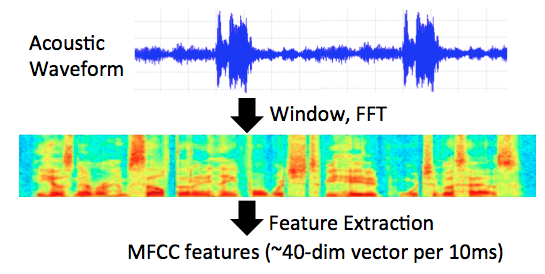
\includegraphics[scale=0.4]{figs/spectogram}
\ei
\end{frame}

\begin{frame}
\frametitle{DNN-HMM Hybrid Architecture}
\be
\item Train Deep Belief Nets on speech features: typically 3-8 layers, 2000 units/layer, 15 frames of input, 6000 output
\item Fine-tune with frame-per-frame phone labels obtained from traditional Gaussian models
\item Further discriminative training in conjunction with higher-level Hidden Markov Model
\ee
\centerline{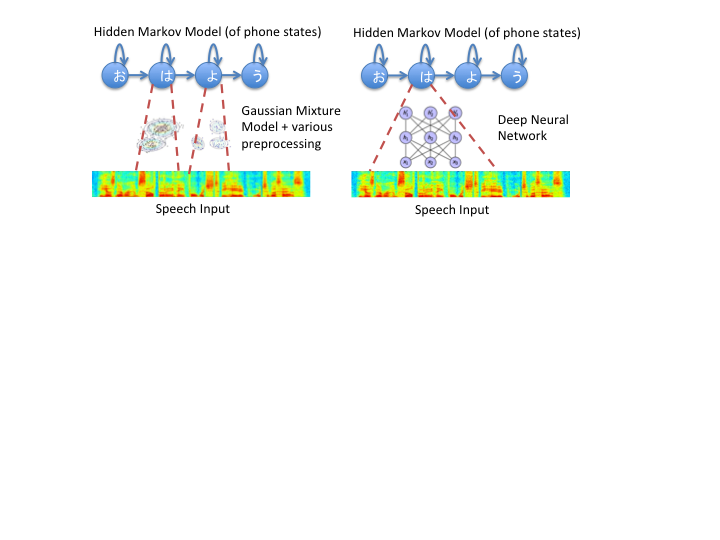
\includegraphics[scale=0.6]{figs/ASR}}
\end{frame}

\begin{frame}
\frametitle{Gaussian-Bernoulli RBM for Continuous Data}
\begin{center}
\begin{tikzpicture}[-,>=stealth',shorten >=1pt,auto,node distance=3cm,
  thick,main node/.style={circle,fill=blue!20,draw,font=\sffamily\Large\bfseries}]

  \node[main node] (x1) at (0,0) {$x_1$};
  \node[main node] (x2) at (2,0) {$x_2$};
  \node[main node] (x3) at (4,0) {$x_3$};
  \node[main node] (h1) at (0,2) {$h_1$};
  \node[main node] (h2) at (2,2) {$h_2$};
  \node[main node] (h3) at (4,2) {$h_3$};

  \path[every node/.style={font=\sffamily\small}]
    (x1) edge node {} (h1)
    (x1) edge node {} (h2)
    (x1) edge node {} (h3)
    (x2) edge node {} (h1)
    (x2) edge node {} (h2)
    (x2) edge node {} (h3)
    (x3) edge node {} (h1)
    (x3) edge node {} (h2)
    (x3) edge node {} (h3);
\end{tikzpicture}
\end{center}

$h_j$ are binary, $x_i$ are continuous variables\\
$p(x,h) = \frac{1}{Z_\theta} \exp{( - E_\theta(x,h))} = \frac{1}{Z_\theta}\exp{\left(\sum_i \frac{-(x_i-b_i)^2}{2v_i}  + \sum_{ij} \frac{x_i w_{ij} h_j}{\sqrt{v_i}} + d^T h \right)}$\\
$p(h_j=1|x) = \sigma(\sum_i \frac{w_{ij} x_i}{\sqrt{v_i}} + d_j) $\\
$p(x_i|h)\sim$ Gaussian with mean $b_i+\sqrt{v_i}\sum_j w_{ij} h_j$ and variance $v_i$\\[0.4cm]
Usually, $x$ is normalized to zero mean, unit variance beforehand
\end{frame}



\begin{frame}
\frametitle{GMM vs. DNN in modeling speech}
\bi
\item Speech is produced by modulating a small number of parameters in a dynamical system (e.g vocal tract)
	\bi
	\item True structure should be in low-dimensional space
	\ei
\pause
\item GMM's: $p(x)=\sum_j p(h_j)p(x|h_j)$ with $p(x|h_j)$ as Gaussian
	\bi
	\item High model expressiveness: can model any non-linear data
	\item But may require large {\bf full}-covariance Gaussians or {\bf many} diagonal-covariance Gaussians $\rightarrow$ statistically inefficient
	\ei
\ei
\centerline{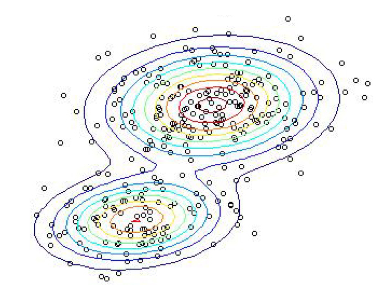
\includegraphics[scale=0.3]{figs/gaussianmixture}}
\pause
\bi
\item RBM \& DNN's distributed factor representation is more efficient 
	\bi
	\item Also: no need to worry about feature correlation $\rightarrow$ exploit larger temporal window as input
	\ei
\ei

\end{frame}


\begin{frame}
\frametitle{Results}
DNN-HMM outperforms GMM-HMM on various datasets\\
Already commercialized!\\[1cm]

Word Error Rate Results:

\centerline{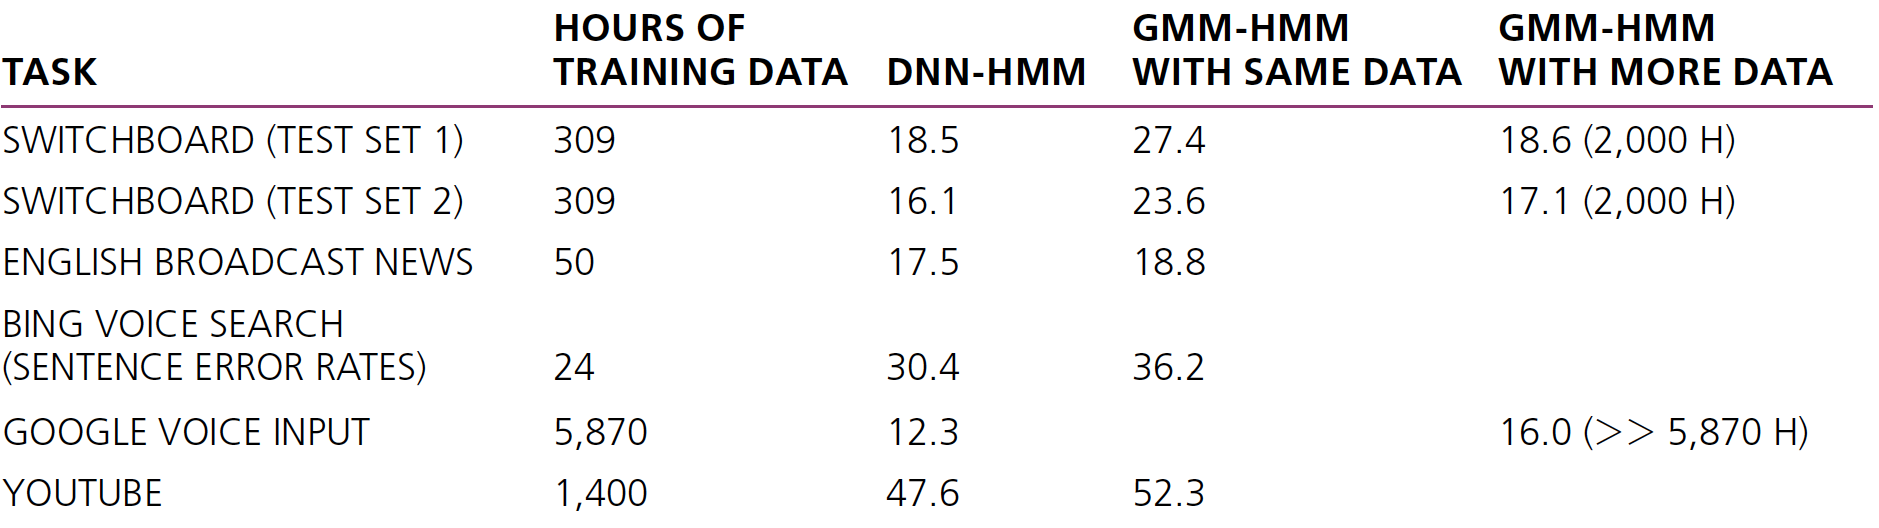
\includegraphics[scale=0.18]{figs/hinton12wer}}

Why it works: Larger context and less hand-engineered preprocessing\\

\end{frame}


\begin{frame}
\frametitle{More details on Switchboard result \cite{seide11speech}}
Basic Setup:
\bi
\item Input: 39-dim derived from PLP, HLDA transform
\item Output: 9304 cross-word triphone states (tied)
\ei
Baseline GMM-HMM:
\bi
\item GMM with 40 Gaussians.	
\item Training: (1) max-likelihood (EM), (2) discriminative BMMI
\ei
DNN-HMM:
\bi
\item 7 stacked RBM's with 2048 units per layer
\item Pre-training on 2 passes over training data (300 hours of speech)
\item Mini-batch size:100-300 (pre-training), 1000 (backpropagation)
\ei
\centerline{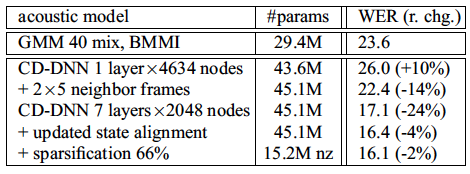
\includegraphics[scale=0.45]{figs/seide11results}}
\end{frame}

%%%%%%%%%%%%%%%%%


%%%%%%%%%
\begin{frame}
\frametitle{Today's Topic}
\tableofcontents
\end{frame}

%SECTION%%%%%%%%%%%%%%%%%%%
\section{Building High-Level Features using Large Scale Unsupervised Learning \cite{le12highlevel}}
%%%%%%%%%%%%%%%%%%%%

%% SUBSECTION%%%%%
%\subsection[Motivation]{Motivation}

%%%%%%%%%%%
\begin{frame}
\frametitle{Motivating Question: Is it possible to learn high-level features (e.g. face detectors) using only unlabeled images?}
\bi
\pause
\item Answer: yes. 
\pause
\bi
\item Using a deep network of 1 billion parameters
\item 10 million images (sampled from Youtube)
\item 1000 machines (16,000 cores) x 1 week.
\ei
\ei
\end{frame}

%%%%%%%%%%%
\begin{frame}
\frametitle{"Grandmother Cell" Hypothesis}
\bi
\item Grandmother cell: A neuron that lights up when you see or hear your grandmother
	\bi
	\item Lots of interesting (controversial) discussions in the neuroscience literature
	\ei
\item For our purposes: is it possible to learn such high-level concepts from raw pixels?
\ei
\end{frame}

%% SUBSECTION%%%%%
%\subsection[Architecture]{Architecture}

\begin{frame}
\frametitle{Previous work: Convolutional Nets \cite{lecun98conv}}
\begin{columns}[c]
    \column{.5\textwidth}
\scalebox{0.7}{\begin{tikzpicture}[->,>=stealth',shorten >=1pt,auto,node distance=3cm,
  thick,main node/.style={circle,fill=blue!20,draw,font=\sffamily\Large\bfseries}]

  \node[main node] (x1) at (0,0) {$x_1$};
  \node[main node] (x2) at (2,0) {$x_2$};
  \node[main node] (x3) at (4,0) {$x_3$};
  \node[main node] (x4) at (6,0) {$x_4$};
  \node[main node] (x5) at (8,0) {$x_5$};
  \node[main node] (h1) at (2,2) {$h_1$};
  \node[main node] (h2) at (4,2) {$h_2$};
  \node[main node] (h3) at (6,2) {$h_3$};
  \node[main node] (h'1) at (3,4) {$p_1$};
  \node[main node] (h'2) at (5,4) {$p_2$};

  \path[every node/.style={font=\sffamily\small}]
    (x1) edge node {} (h1)
    (x2) edge node {} (h1)
    (x3) edge node {} (h1)
    (x2) edge node {} (h2)
    (x3) edge node {} (h2)
    (x4) edge node {} (h2) 
    (x3) edge node {} (h3)
    (x4) edge node {} (h3)
    (x5) edge node {} (h3)
    (h1) edge node {} (h'1)
    (h2) edge node {} (h'1)
    (h2) edge node {} (h'2)
    (h3) edge node {} (h'2)
    ;
\end{tikzpicture}}
    \column{.5\textwidth}
{\bf Receptive Field (RF)}: each $h_j$ only connects to small input region.\\
Tied weights $\rightarrow$ convolution\\
{\bf Pooling}: e.g. $p_1=max(h_1,h_2)$ or $p_1=\sqrt{h_1^2+h_2^2}$\\[0.2cm]
Advantages: 
\be
\item Fewer weights
\item Shift invariance
\ee
\end{columns}
\pause
\begin{center}
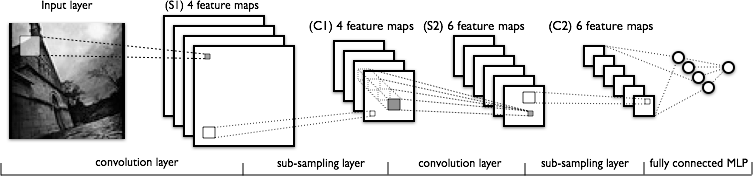
\includegraphics[scale=0.6]{figs/lenet}\\
\small{(Figure from \url{http://deeplearning.net/tutorial/lenet.html})}
\end{center}
\end{frame}

\begin{frame}
\frametitle{Architecture}
\begin{columns}[c]
    \column{.5\textwidth}
	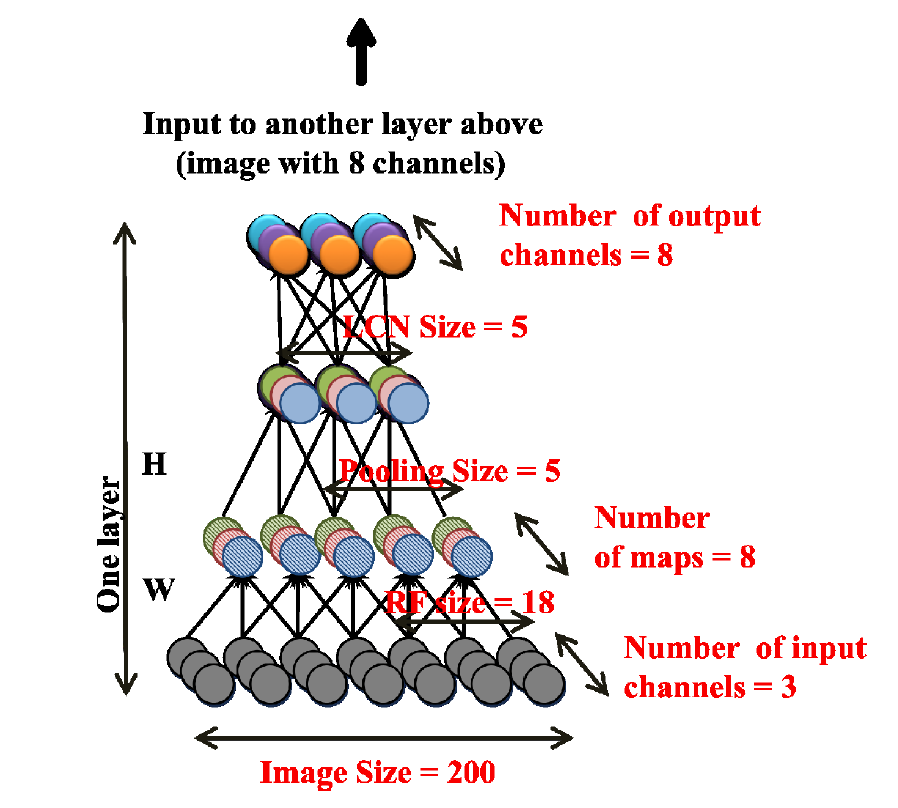
\includegraphics[scale=0.25]{figs/le12architecture}
    \column{.5\textwidth}
	\begin{eqnarray}
	\min_{W_d,W_e} \sum_m ||W_d W_e x^{(m)} - x^{(m)} ||  \\
	+ \sum_{m,k} \sqrt{\epsilon + P_k (W_e x^{(m)})^2}  
	\end{eqnarray}
	\hspace{2cm} (1): auto-encoder \\
	\hspace{2cm} (2): pooling
\end{columns}
Repeated 3 times to form Deep Architecture\\
$x^{(m)}=$ image of 200x200 pixels x3 channels
\end{frame}


\begin{frame}
\frametitle{Feature learning by Topographic ICA \cite{hyvarinen01tica}}
Learns shift/scale/rotation-invariant features
\begin{columns}[c]
    \column{.5\textwidth}
	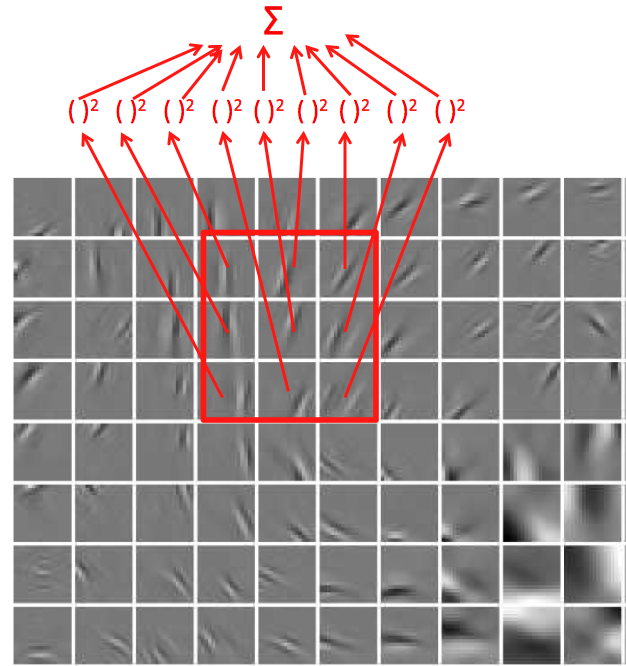
\includegraphics[scale=0.25]{figs/topographic_ica}
    \column{.5\textwidth}
	     Reconstruction version \cite{le11rica} can be trained faster
	\begin{eqnarray}
	\min_{W_d,W_e} \sum_m ||W_d W_e x^{(m)} - x^{(m)} || \nonumber  \\
	+ \sum_{m,k} \sqrt{\epsilon + P_k (W_e x^{(m)})^2}  \nonumber
	\end{eqnarray}
\end{columns}
\end{frame}

\begin{frame}
\frametitle{Training Setup}
\bi
\item 3-layer network, 1 billion parameters (trained jointly)
\item 10 million 200x200 pixel images from 10 million Youtube videos
\item 1000 machines (16,000 cores) x 1 week
\item Lots of tricks for data/model parallelization (next lecture)
\ei
\end{frame}


%% SUBSECTION%%%%%
%\subsection[Results]{Experimental Results}

\begin{frame}
\frametitle{Face neuron}
\centerline{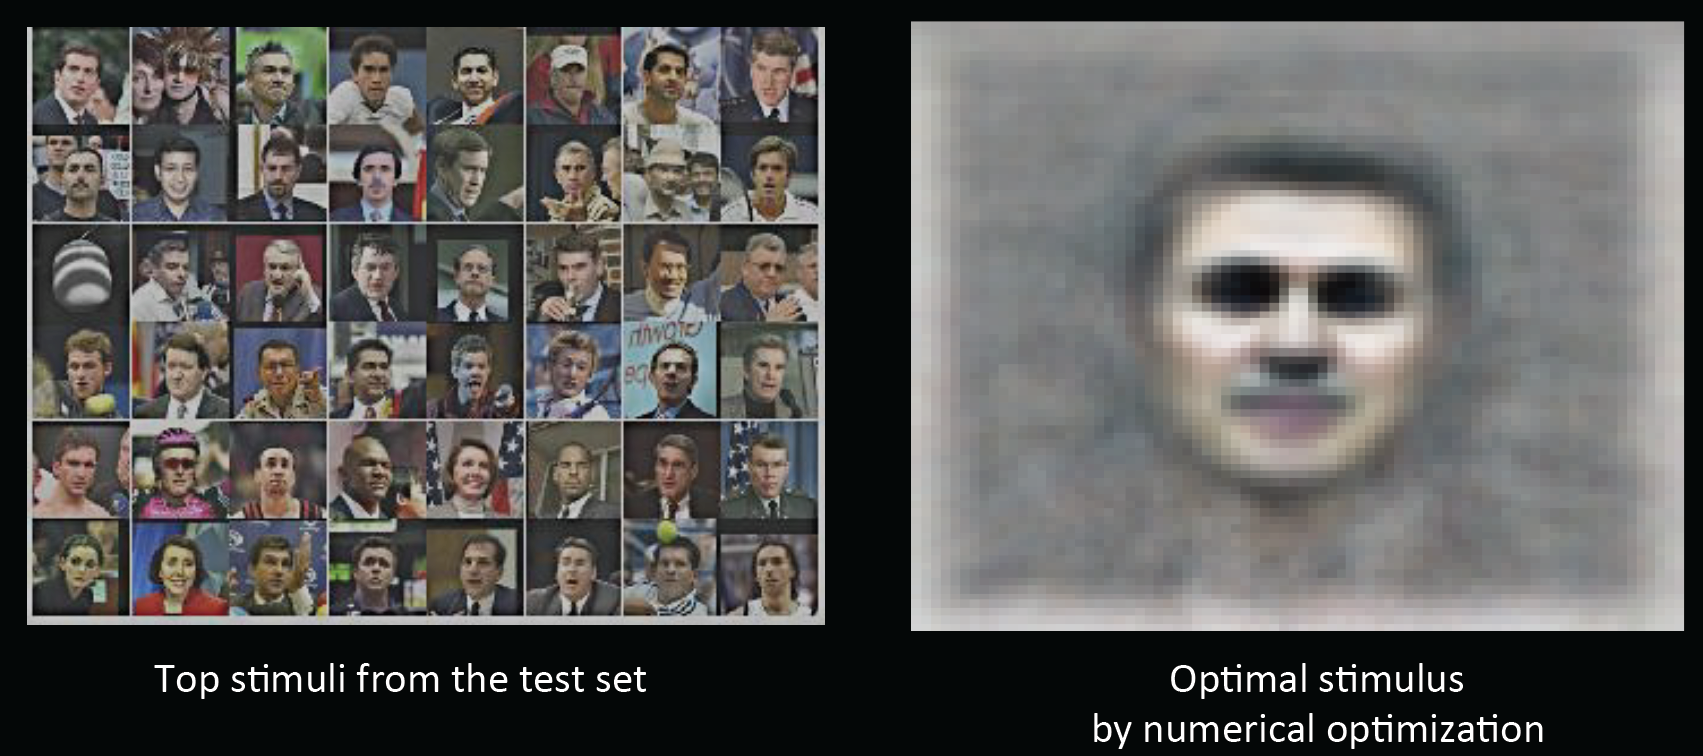
\includegraphics[scale=0.2]{figs/le12face}}
*Graphics from \cite{le12highlevel}
\end{frame}

\begin{frame}
\frametitle{Face neuron}
\centerline{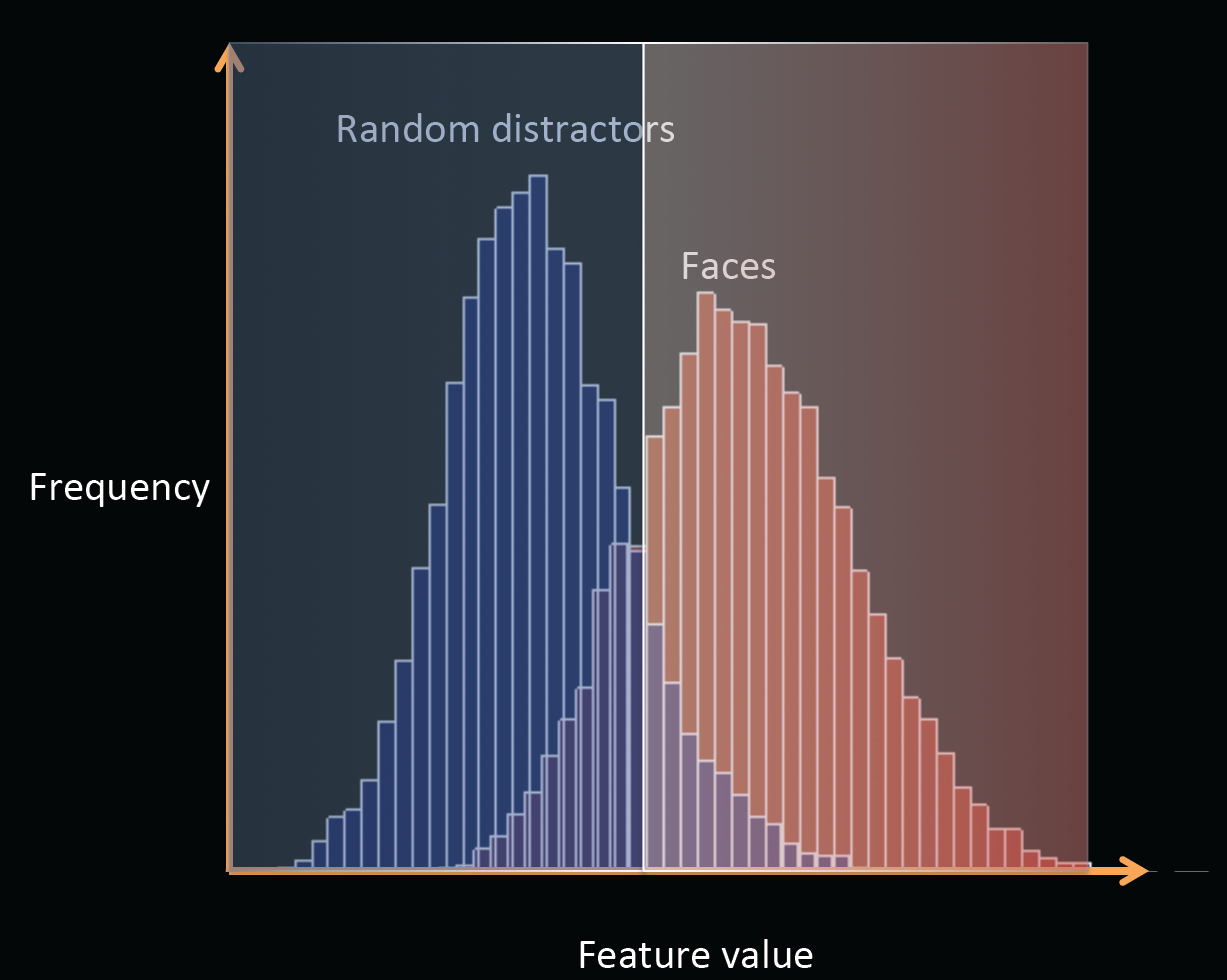
\includegraphics[scale=0.2]{figs/le12face_histogram}}
*Graphics from \cite{le12highlevel}
\end{frame}

\begin{frame}
\frametitle{Cat neuron}
\centerline{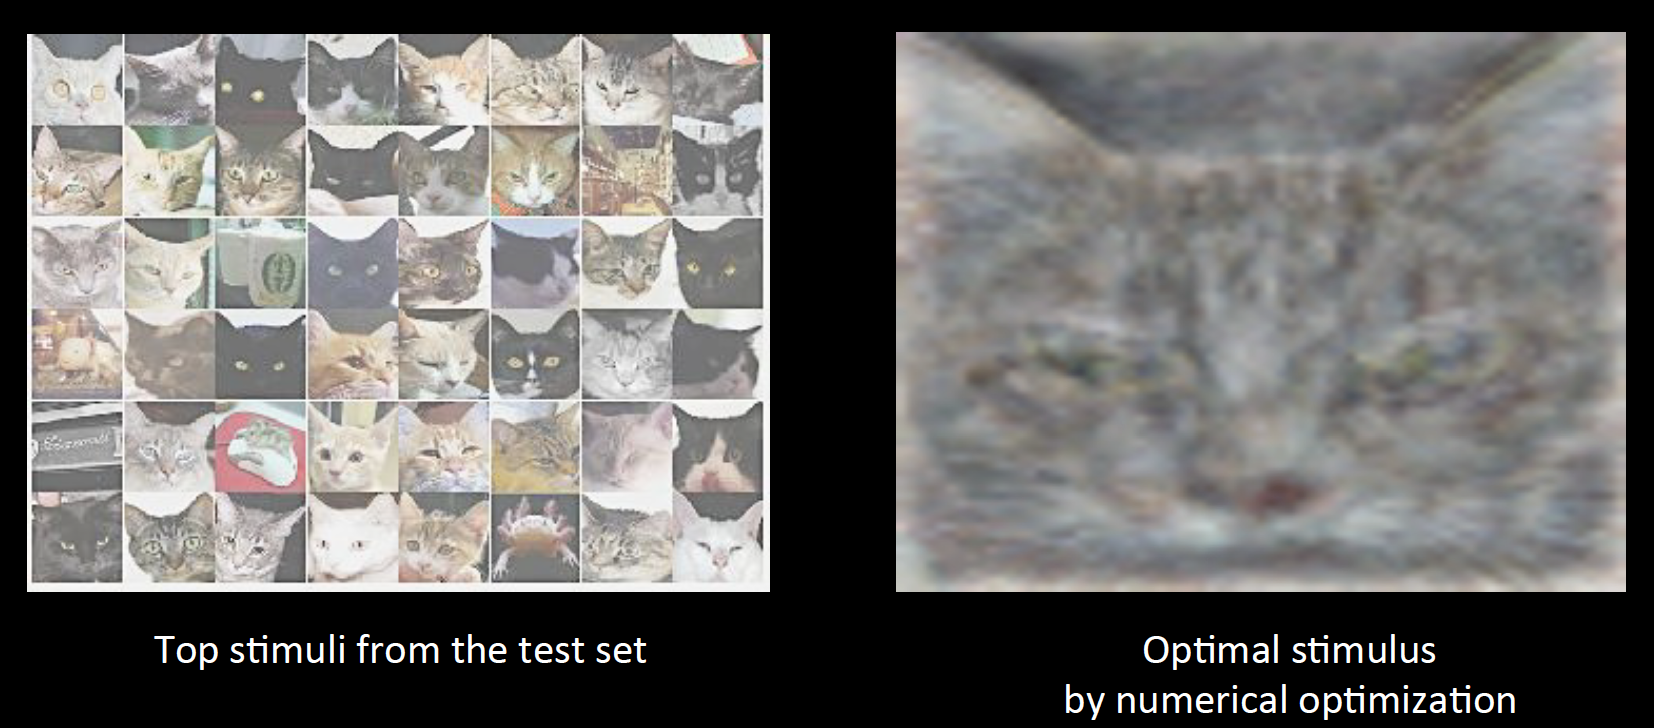
\includegraphics[scale=0.2]{figs/le12cat}}
*Graphics from \cite{le12highlevel}
\end{frame}

\begin{frame}
\frametitle{More examples}
\centerline{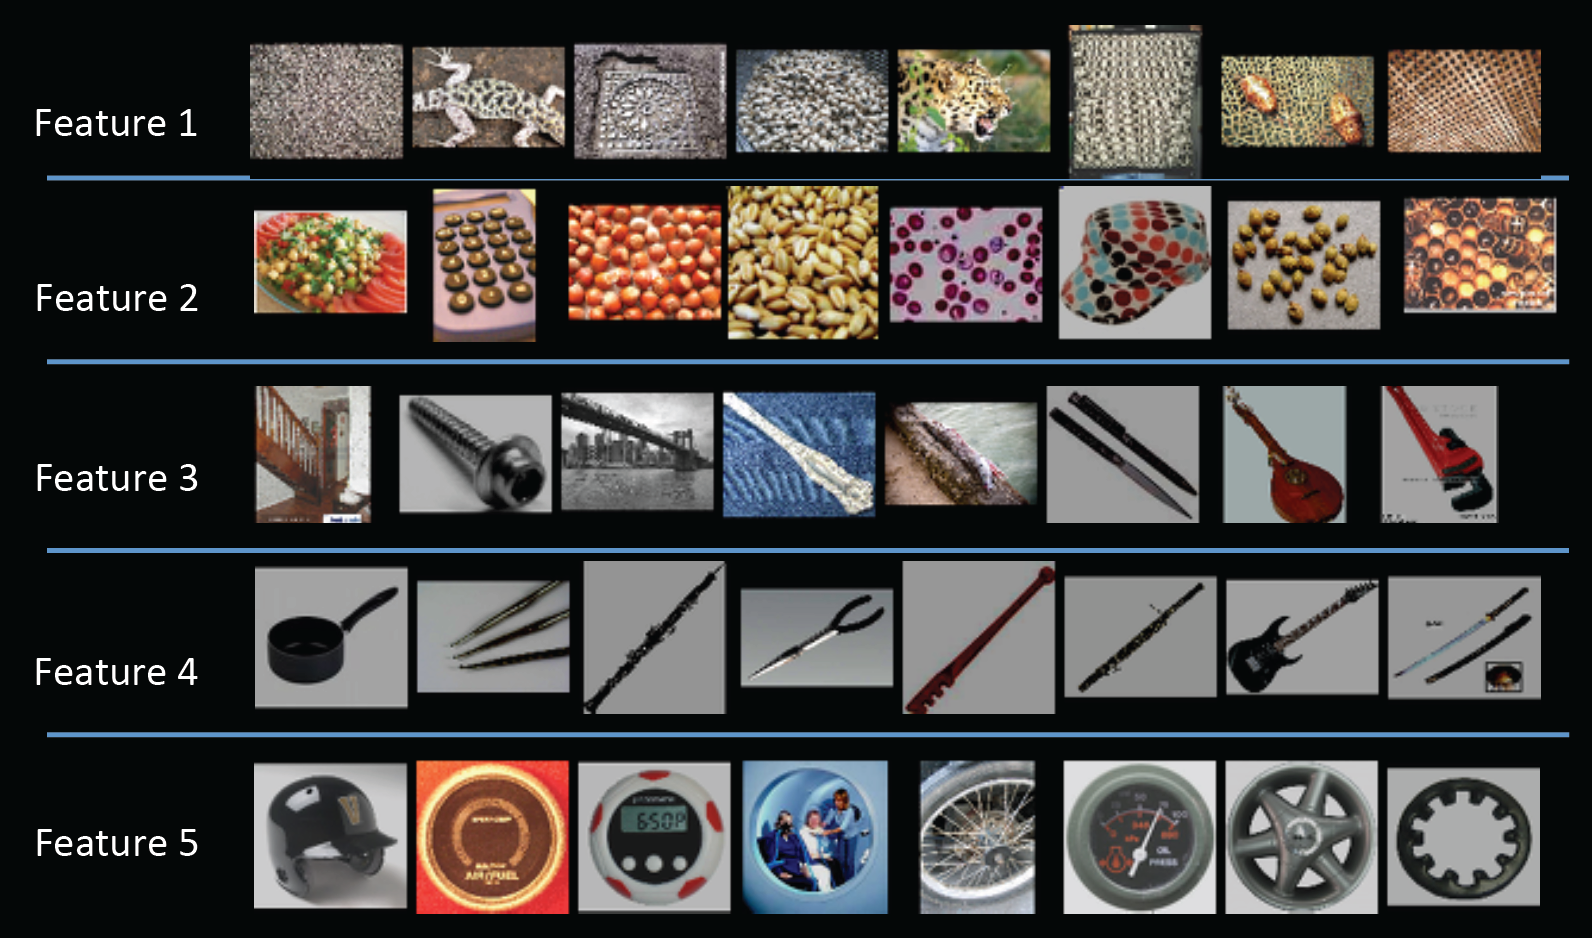
\includegraphics[scale=0.2]{figs/le12examples1}}
*Graphics from \cite{le12highlevel}
\end{frame}

\begin{frame}
\frametitle{More examples}
\centerline{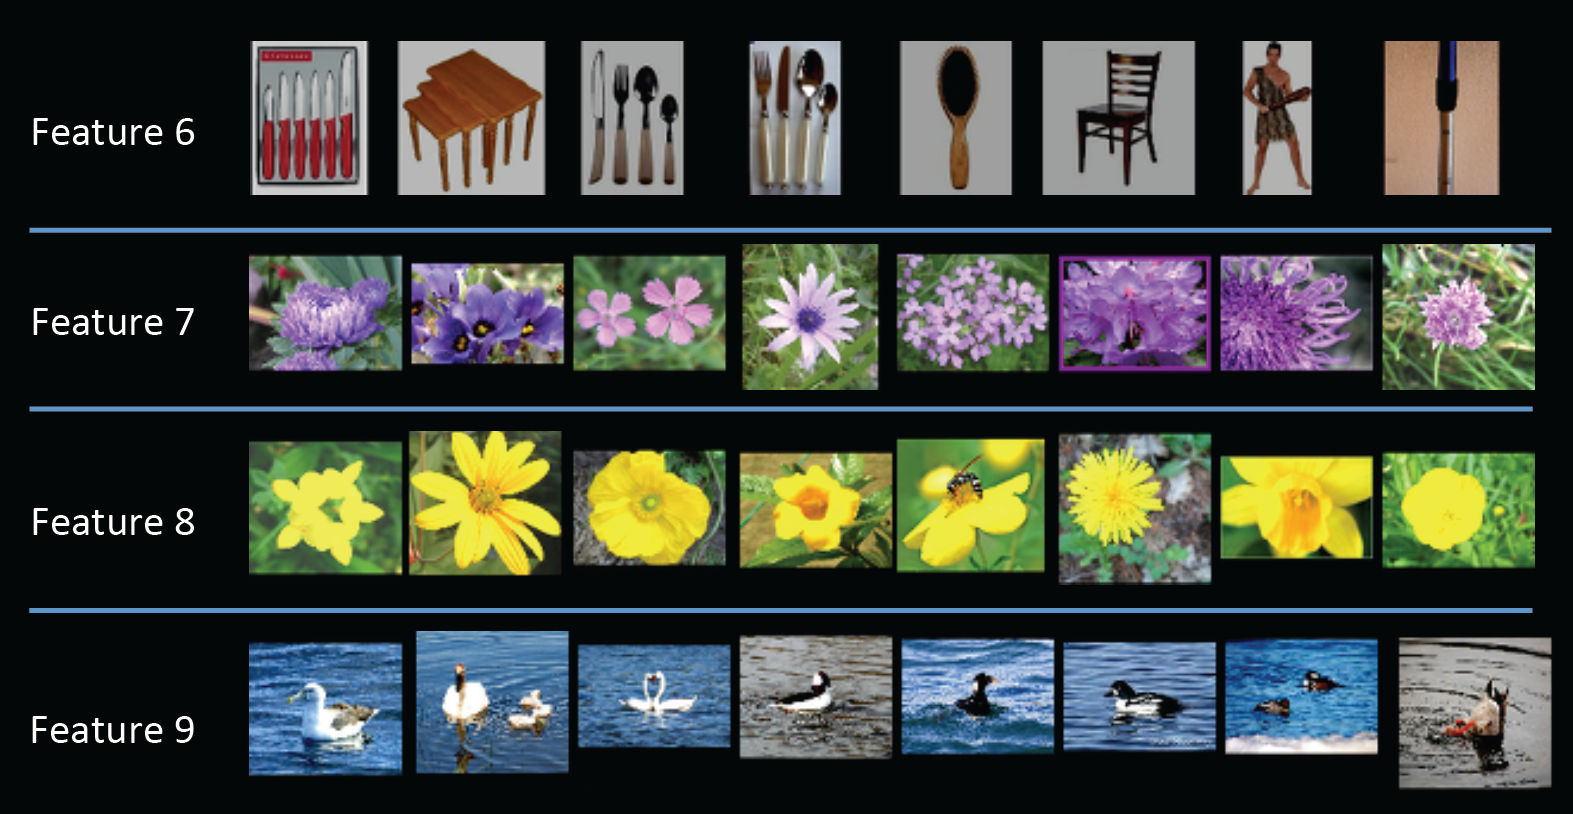
\includegraphics[scale=0.2]{figs/le12examples2}}
*Graphics from \cite{le12highlevel}
\end{frame}

\begin{frame}
\frametitle{More examples}
\centerline{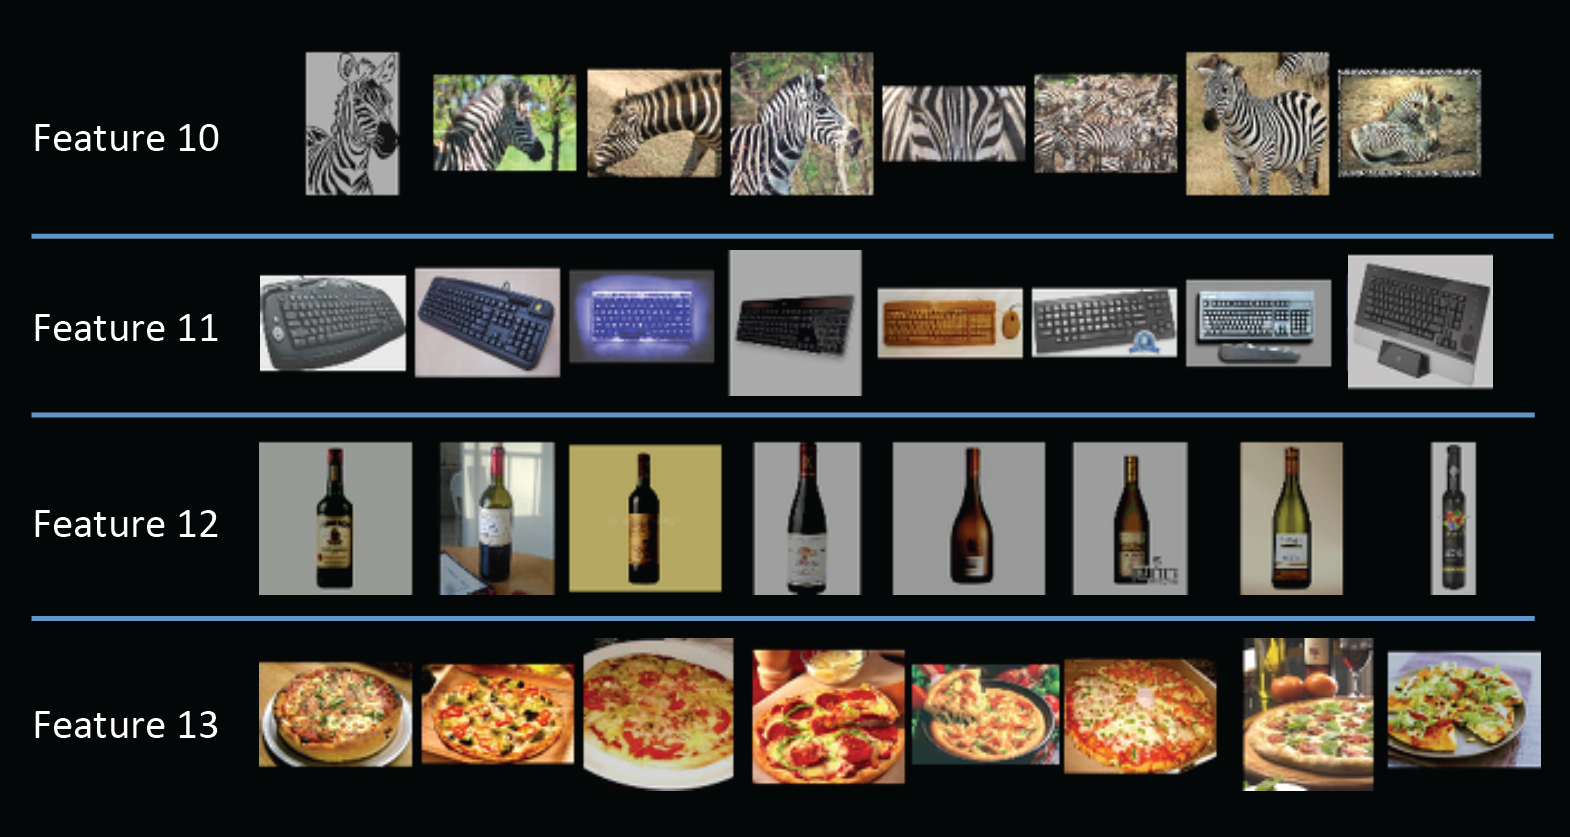
\includegraphics[scale=0.2]{figs/le12examples3}}
*Graphics from \cite{le12highlevel}
\end{frame}

\begin{frame}
\frametitle{ImageNet Classification Results}
\centerline{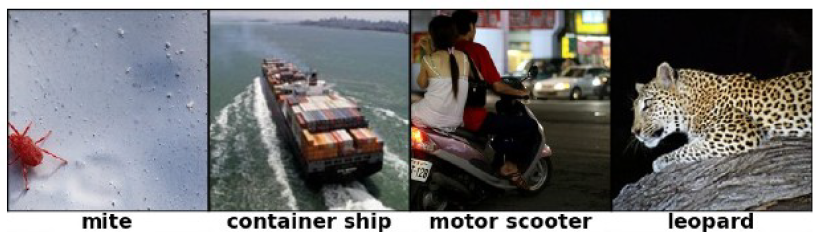
\includegraphics[scale=0.4]{figs/imagenet}}
\bi
\item Add logistic regression on top of final layer
\item Supervised learning on ImageNet dataset
\ei

Test Accuracy (22K categories):\\
\begin{tabular}{|l|c|}
\hline
Method & Accuracy \\ \hline
Random & 0.005\% \\
Previous State-of-the-art & 9.3\% \\
\cite{le12highlevel} without pre-training on Youtube data & 13.6\% \\
\cite{le12highlevel} with pre-training on Youtube data & 15.8\% \\
\hline
\end{tabular}
\end{frame}

%%%%%%%%%
\begin{frame}
\frametitle{Today's Topic}
\tableofcontents
\end{frame}

%SECTION%%%%%%%%%%%%%%%%%%%
\section{Recurrent Neural Network Language Models \cite{mikolov10rnnlm}}
%%%%%%%%%%%%%%%%%%%%

\begin{frame}
\frametitle{Goal of Language Modeling}
\bi
\item Give probabilities to word sequences (e.g. sentences)
\bi
	\item Likely sentences in the world (e.g. "let's recognize speech") $\rightarrow$ high probability
	\item Unlikely sentences in the world (e.g. "let's wreck a nice beach") $\rightarrow$ low probability
\ei
\item Useful for various applications involving natural language
\pause
\item N-gram model decomposes sentence probability, e.g. $p(w^{(1)},w^{(2)},w^{(3)},w^{(4)})=$
\bi
\item $p(w^{(4)}|w^{(3)})p(w^{(3)}|w^{(2)})p(w^{(2)}|w^{(1)})p(w^{(1)})$ (2-gram)
\item $p(w^{(4)}|w^{(3)},w^{(2)})p(w^{(3)}|w^{(2)},w^{(1)})p(w^{(2)}|w^{(1)})p(w^{(1)})$ (3-gram)
\ei
\pause
\item Estimate from text data: $p(w^{(2)}|w^{(1)}) = count(w^{(1)},w^{(2)})/count(w^{(1)}) $, plus smoothing to account for unknown words and word sequences
\ei
\end{frame}

\begin{frame}
\frametitle{Recurrent Neural Net Architecture for Language Modeling}
Model $p(current\_word|previous\_words)$ with a recurrent hidden layer

\begin{columns}
\column{0.6\textwidth}
\scalebox{0.7}{\begin{tikzpicture}[->,>=stealth',shorten >=1pt,auto,node distance=3cm,
  thick,main node/.style={circle,fill=blue!20,draw,font=\sffamily\Large\bfseries}]

  \node[main node] (x1) at (0,0) {$x_1$};
  \node[main node] (x2) at (2,0) {$x_2$};
  \node[main node] (x3) at (4,0) {$x_3$};
  \node[main node] (x4) at (6,0) {$x_4$};
  \node[main node] (x5) at (8,0) {$x_5$};
  \node[main node] (h1) at (4,2) {$h_1$};
  \node[main node] (h2) at (6,2) {$h_2$};
  \node[main node] (h'1) at (0,4) {$y_1$};
  \node[main node] (h'2) at (2,4) {$y_2$};
  \node[main node] (h'3) at (4,4) {$y_3$};

  \draw[blue,ultra thick,-latex,<->] (0,-1) -- node[]{Previous Word} (4,-1);
  \draw[blue,ultra thick,-latex,<->] (6,-1) -- node[]{Previous $h$} (8,-1);
  \draw[blue,ultra thick,-latex,<->] (0,5) -- node[]{Current Word (assume 3-word vocabulary)} (4,5);

   \node(wij) at (1,1) {$w_{ij}$};
   \node(wjk) at (1,3) {$w_{jk}$};
   
  \path[every node/.style={font=\sffamily\small}]
    (x1) edge node {} (h1)
    (x2) edge node {} (h1)
    (x3) edge node {} (h1)
    (x4) edge node {} (h1)
    (x5) edge node {} (h1)
    (x1) edge node {} (h2)
    (x2) edge node {} (h2)
    (x3) edge node {} (h2)
    (x4) edge node {} (h2)
    (x5) edge node {} (h2)
    (h1) edge node {} (h'1)
    (h2) edge node {} (h'1)
    (h1) edge node {} (h'2)
    (h2) edge node {} (h'2)
    (h1) edge node {} (h'3)
    (h2) edge node {} (h'3)
    ;
\end{tikzpicture}}
    \column{.4\textwidth}
\bi
\item Probability of word k: $y_k=\frac{\exp(W_{jk}^T h)}{\sum_{k'}\exp(W_{jk'}^T h)}$ 
\item $[x_1,x_2,x_3]$ is binary vector with 1 at current vocabulary \& 0 otherwise
\item $[x_4,x_5]$ is a copy of $[h_1,h_2]$ from the previous time-step
\item $h_j=\sigma(W_{ij}^T x_i)$ is hidden "state" of the system
\ei
\end{columns}
\end{frame}

\begin{frame}
\frametitle{Training: Backpropagation through Time}
Unroll the hidden states for certain time-steps.\\
Given error at $y$, update weights by backpropagation

{\color{red} \textit{Example:  he loves $|$ her}}

\scalebox{0.8}{\begin{tikzpicture}[->,>=stealth',shorten >=1pt,auto,node distance=3cm,
  thick,main node/.style={circle,fill=blue!20,draw,font=\sffamily\Large\bfseries}]

  \node[main node] (x1) at (0,0) {$x_1$};
  \node[main node] (x2) at (2,0) {$x_2$};
  \node[main node] (x3) at (4,0) {$x_3$};
  \node[main node] (x4) at (6,0) {$h'_1$};
  \node[main node] (x5) at (8,0) {$h'_2$};
  \node[main node] (h1) at (4,2) {$h_1$};
  \node[main node] (h2) at (6,2) {$h_2$};
  \node[main node] (h'1) at (0,4) {$y_1$};
  \node[main node] (h'2) at (2,4) {$y_2$};
  \node[main node] (h'3) at (4,4) {$y_3$};

  \node[main node] (px1) at (2,-3) {$x_1$};
  \node[main node] (px2) at (4,-3) {$x_2$};
  \node[main node] (px3) at (6,-3) {$x_3$};
  \node[main node] (px4) at (8,-3) {$h''_1$};
  \node[main node] (px5) at (10,-3) {$h''_2$};

  \draw[blue,ultra thick,-latex,<->] (2,-4) -- node[]{"he" $[x_1,x_2,x_3]=[0,1,0]$} (6,-4);
  \draw[blue,ultra thick,-latex,<->] (0,-1) -- node[]{"loves" $[x_1,x_2,x_3]=[1,0,0]$} (4,-1);
 \draw[blue,ultra thick,-latex,<->] (6,-1) -- node[]{Previous $h$} (8,-1);
\draw[blue,ultra thick,-latex,<->] (8,-4) -- node[]{Initial $h$} (10,-4);
   \node(wij) at (1,1) {$w_{ij}$};
   \node(wjk) at (1,3) {$w_{jk}$};
      \node(wij) at (3,-2) {$w_{ij}$};

  \path[every node/.style={font=\sffamily\small}]
    (px1) edge node {} (x4)
    (px2) edge node {} (x4)
    (px3) edge node {} (x4)
    (px4) edge node {} (x4)
    (px5) edge node {} (x4)
    (px1) edge node {} (x5)
    (px2) edge node {} (x5)
    (px3) edge node {} (x5)
    (px4) edge node {} (x5)
    (px5) edge node {} (x5)
    (x1) edge node {} (h1)
    (x2) edge node {} (h1)
    (x3) edge node {} (h1)
    (x4) edge node {} (h1)
    (x5) edge node {} (h1)
    (x1) edge node {} (h2)
    (x2) edge node {} (h2)
    (x3) edge node {} (h2)
    (x4) edge node {} (h2)
    (x5) edge node {} (h2)
    (h1) edge node {} (h'1)
    (h2) edge node {} (h'1)
    (h1) edge node {} (h'2)
    (h2) edge node {} (h'2)
    (h1) edge node {} (h'3)
    (h2) edge node {} (h'3)
    ;
\end{tikzpicture}}
\end{frame}

%%%%
\begin{frame}
\frametitle{Advantages of Recurrent Nets}
\bi
\item Hidden nodes $h$ form a distributed representation of partial sentence
\bi
	\item $h$ is a succinct conditioning factor for predicting current word
	\item Arbitrarily-long history is (theoretically) kept through recurrence
\ei
\pause
\item In practice:
	\bi
	\item Backpropatation through Time forms a deep network; may be hard to train. Fixed to $<10$ previous time-steps/words 
	\item $y_k=\frac{\exp(W_{jk}^T h)}{\sum_{k'}\exp(W_{jk'}^T h)}$ requires summation $k$ over vocabulary size, which is large. There are shortcuts to reduce computation.
	\ei
\pause
\item By-product: $[w_{ij}]_i$ can be used as "word embeddings". Useful for various natural language processing tasks \cite{zhila13,turian10word} 
\ei
\end{frame}


%%%
\begin{frame}
\frametitle{Results \cite{mikolov10rnnlm}}

Trained on 6 million words (300K sentences) of New York Times data.\\[0.2cm] 
Evaluation on held-out data:\\ \hspace{1cm} $perplexity=2^{entropy} = 2^{- \frac{1}{|data|}\sum_{data} \log{p_{model}(data)}}$\\[1cm]

\begin{tabular}{|c|c|}
\hline
{\bf Model} & {\bf Perplexity} \\
\hline\hline
N-gram (N=5) & 221 \\
\hline
Recurrent Net $|h|=60$ & 229\\
Recurrent Net $|h|=90$ & 202\\
Recurrent Net $|h|=250$ & 173\\
Recurrent Net $|h|=400$ & 171\\
\hline
Combining 3 Recurrent Nets & 151 \\
Combining 3 Recurrent Nets, dynamic update on held-out & 128 \\
\hline
\end{tabular}
\end{frame}


\begin{frame}[allowframebreaks]
\frametitle{References}
\bibliographystyle{apalike}
\bibliography{mybib}
\end{frame}

\end{document}
